\documentclass[letterpaper, 12pt]{article}

\usepackage{geometry}
 \geometry{
 letterpaper,
 total={170mm,257mm},
 left=20mm,
 top=20mm,
 bottom=20mm
 }
\usepackage{graphicx} % Required for inserting images
\usepackage{authblk}
\usepackage{amssymb}
\usepackage{lipsum}
\usepackage{float}
\usepackage{times}
\usepackage{amsmath}
\usepackage[format=plain,
            labelfont={bf,it},
            textfont=it]{caption}
\captionsetup{justification=raggedright,singlelinecheck=false}
\usepackage{ragged2e}
\usepackage{longtable}
\usepackage{comment}
\usepackage{setspace}
\usepackage{fancyhdr}
\usepackage{titlesec}
\usepackage[hyperindex,breaklinks]{hyperref}
\hypersetup{
    colorlinks=true,
    linkcolor=blue,
    filecolor=magenta,      
    urlcolor=blue
    }
% \usepackage{background} % add COSIG logo to page
\usepackage[T1]{fontenc}
\usepackage{helvet}
\renewcommand{\familydefault}{\sfdefault}
\pagenumbering{gobble}
\usepackage[skip=10pt plus1pt, indent=40pt]{parskip}

\titlespacing*{\section}
{0pt}{1.5ex plus 1ex minus .2ex}{1.3ex plus .2ex}

\renewcommand\Authfont{\fontsize{12}{14.4}\selectfont}
\renewcommand\Affilfont{\fontsize{9}{10.8}\itshape}
 
\begin{document}
\flushleft

\includegraphics[width=0.5\textwidth]{img/home/241017_final_logo_mockup.png}

\section*{X-ray diffraction patterns - data duplication}
\addcontentsline{toc}{section}{X-ray diffraction patterns - data duplication}
\textit{Last updated: 19 May 2025}

Data duplication refers to the practice of using the same data to represent different things. Readers don't usually have access to the raw data appearing in an article's figures and thus data duplication can often be difficult to spot. Furthermore, image forensics tools designed to find duplicated images will often not spot duplications in other data formats.

Data duplication is relatively easy to spot in X-ray diffraction (XRD) patterns because the signal collected from an XRD instrument will usually feature a high-frequency noise component (i.e., the ``fuzz'' on top of an XRD pattern). No matter what, no two XRD patterns will feature the same noise pattern, even if they are collected from the same sample on the same instrument with the same settings.

\begin{figure}[h!tbp]
    \centering
    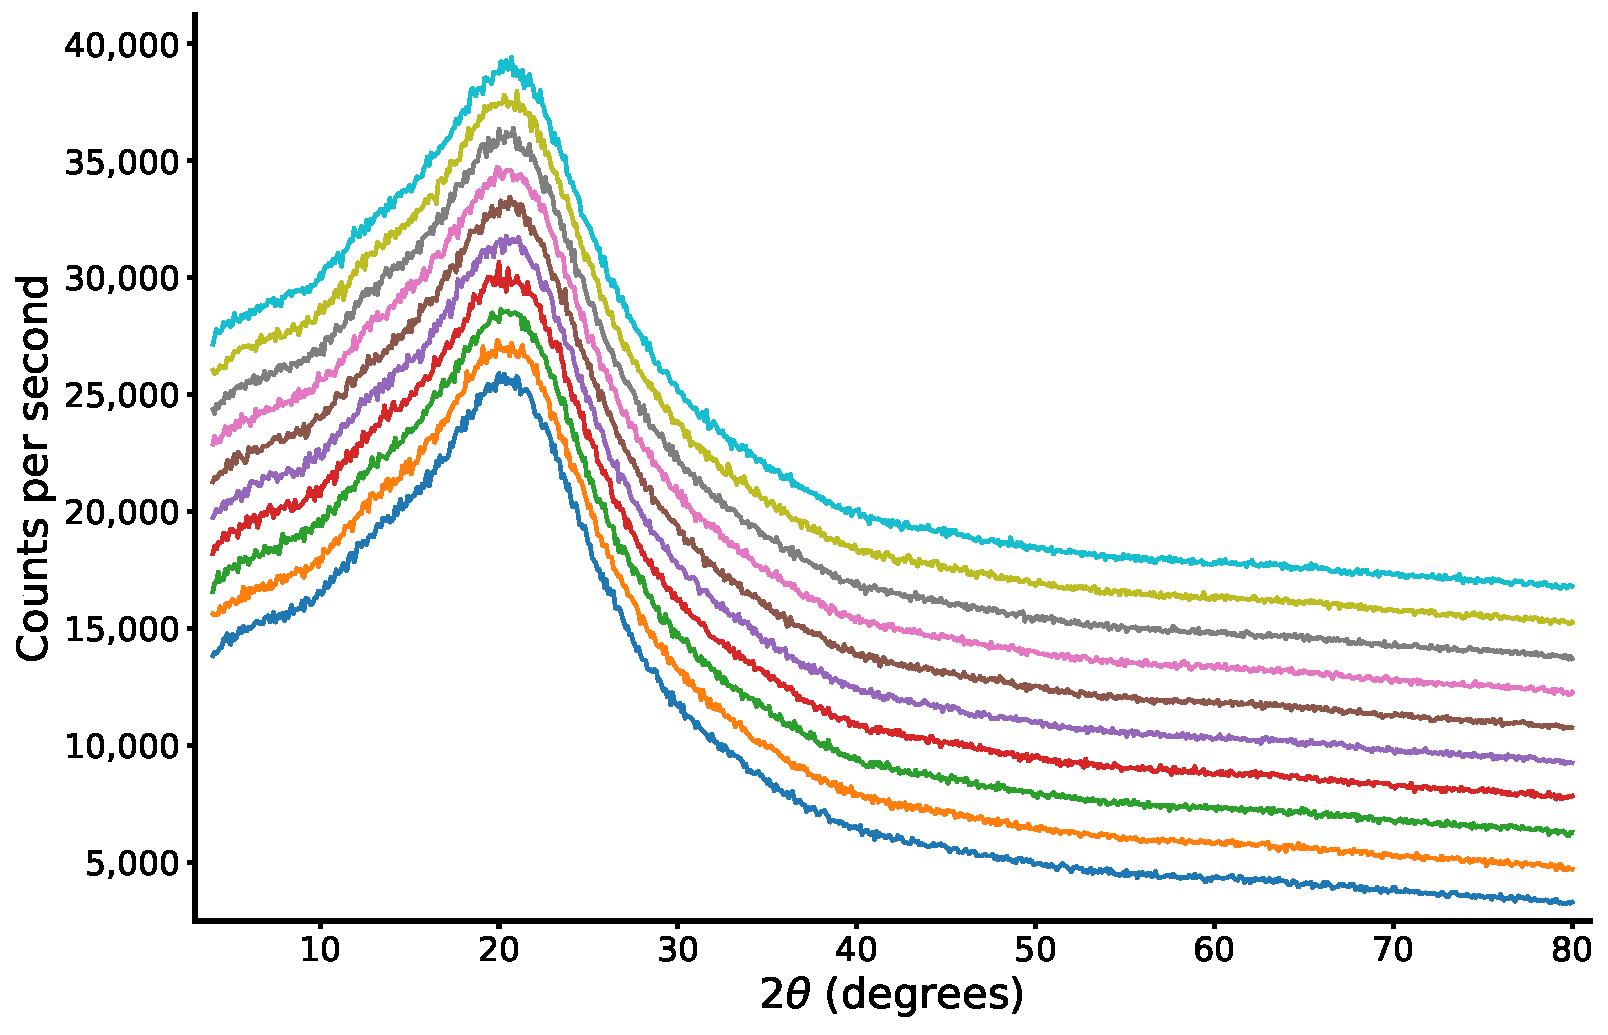
\includegraphics[width=\textwidth]{img/xrd_data_duplication/250519_xrd_x10.pdf}
    \caption*{Ten powder XRD patterns produced from the same sample (a 1.5 mm quartz capillary) on the same instrument (a Rigaku Smartlab) under the same settings (in transmission mode), each collected immediately after the other. Although each pattern is very similar to the others, no two are exactly alike. Traces are vertically displaced for readibility. Data collected at the \href{https://www.xray.facilities.northwestern.edu/}{Northwestern University Jerome B. Cohen X-ray Diffraction Facility}.}
\end{figure}

\subsection*{Example 1: Identical XRD patterns used to represent different materials in the same article}

\href{https://doi.org/10.1007/s10971-023-06078-x}{Benkhelifa et al. (2023)} report on the synthesis of antimony-doped aluminum oxide crystals. However, the XRD patterns shown in Figure 2 for doped and undoped crystals are exactly identical to one another and thus cannot represent different materials.

\begin{figure}[h!tbp]
    \centering
    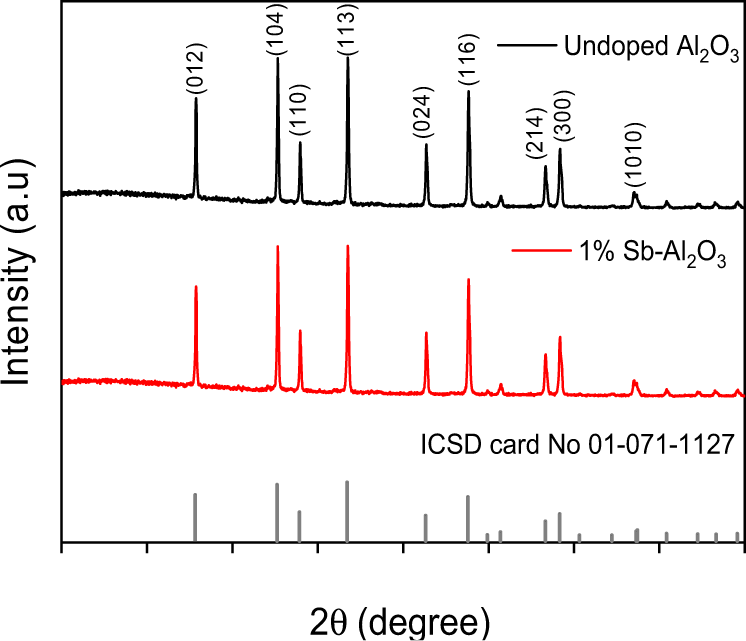
\includegraphics[width=\textwidth]{img/xrd_data_duplication/benkhelifa_figure_2.png}
    \caption*{Adapted from Figure 2 of \href{https://doi.org/10.1007/s10971-023-06078-x}{Benkhelifa et al. (2023)}.}
\end{figure}

\pagebreak

\subsection*{Example 2: Identical XRD pattern used to represent different materials in different articles}

\href{https://doi.org/10.1016/j.jlumin.2016.07.051}{Mahraz et al. (2016)} report on the synthesis and heat treatment of erbium-zinc-boro-tellurite glasses. Figure 1 shows XRD patterns apparently collected from the glass samples after various durations of heat treatment. However, all four XRD patterns shown are exactly identical. In fact, this same XRD pattern has been used in \href{https://pubpeer.com/publications/27A40862805C08DD269520435EAC67\#1}{at least 8 different articles to represent as many as 28 different materials}.

\begin{figure}[h!tbp]
    \centering
    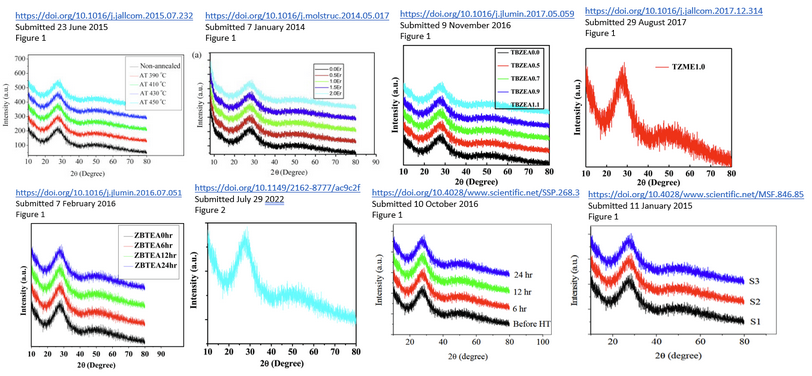
\includegraphics[width=\textwidth]{img/xrd_data_duplication/same_xrd_different_articles_small.png}
    \caption*{Adapted from a figure created by \href{https://pubpeer.com/publications/8A1A8F322680DFB05011853190C254\#1}{Reese Richardson on PubPeer}.}
\end{figure}

\pagebreak

\subsection*{Example 3: Unusually similar XRD patterns used to represent different materials}

\href{https://doi.org/10.1007/s10853-015-9003-3}{Mohaghegh et al. (2015)} report on synthesizing hybrid silver oxide copper terephthalate metal-organic frameworks. However, in Figure 2, the XRD patterns for Ag/MOF and Ag$_\text{2}$O/MOF have identical noise patterns, only differing by the addition of a few peaks. This is highly unlikely to occur by chance. 

\begin{figure}[h!tbp]
    \centering
    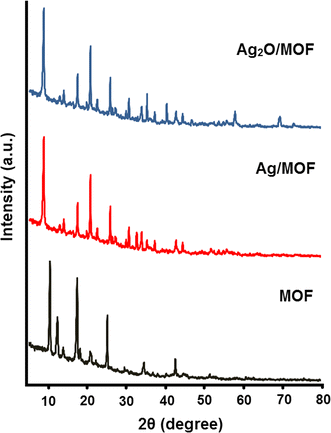
\includegraphics[width=0.4\textwidth]{img/xrd_data_duplication/mohaghegh_figure_2.png}
    \caption*{The XRD patterns for Ag/MOF (red) and Ag$_\text{2}$O/MOF (blue) are identical from 5 to about 33 degrees and thereafter are highly similar except for the addition of several peaks in the Ag$_\text{2}$O/MOF pattern. Adapted from Figure 2 of \href{https://doi.org/10.1007/s10853-015-9003-3}{Mohaghegh et al. (2015)}.}
\end{figure}

\begin{figure}[h!tbp]
    \centering
    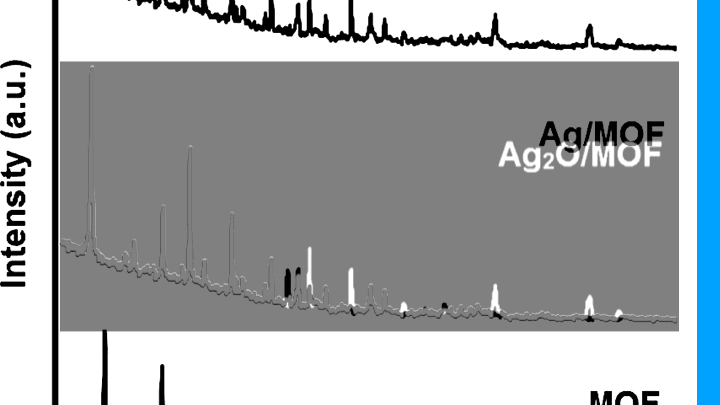
\includegraphics[width=0.4\textwidth]{img/xrd_data_duplication/mohaghegh_figure_2_animation.png}
    \caption*{An overlay of the Ag/MOF and Ag$_\text{2}$O/MOF patterns, demonstrating the unusually high similarity of the patterns' noise profiles. Adapted from an animation by \href{https://pubpeer.com/publications/7BE7C2A93C385F700F1C6B5BC90294\#8}{Illex illecebrosus on PubPeer}.}
\end{figure}

\pagebreak

\subsection*{Example 4: Regions of identical noise in XRD patterns}

\href{https://doi.org/10.1016/j.ijbiomac.2018.09.215}{Abasian et al. (2019)} report of the synthesis of zeolite nanocomposites for drug delivery. However, the XRD patterns shown for the synthesized materials in Figure 1 have several regions of repetitive noise. It is highly unlikely that these repetitive noise patterns arose by chance.

\begin{figure}[h!tbp]
    \centering
    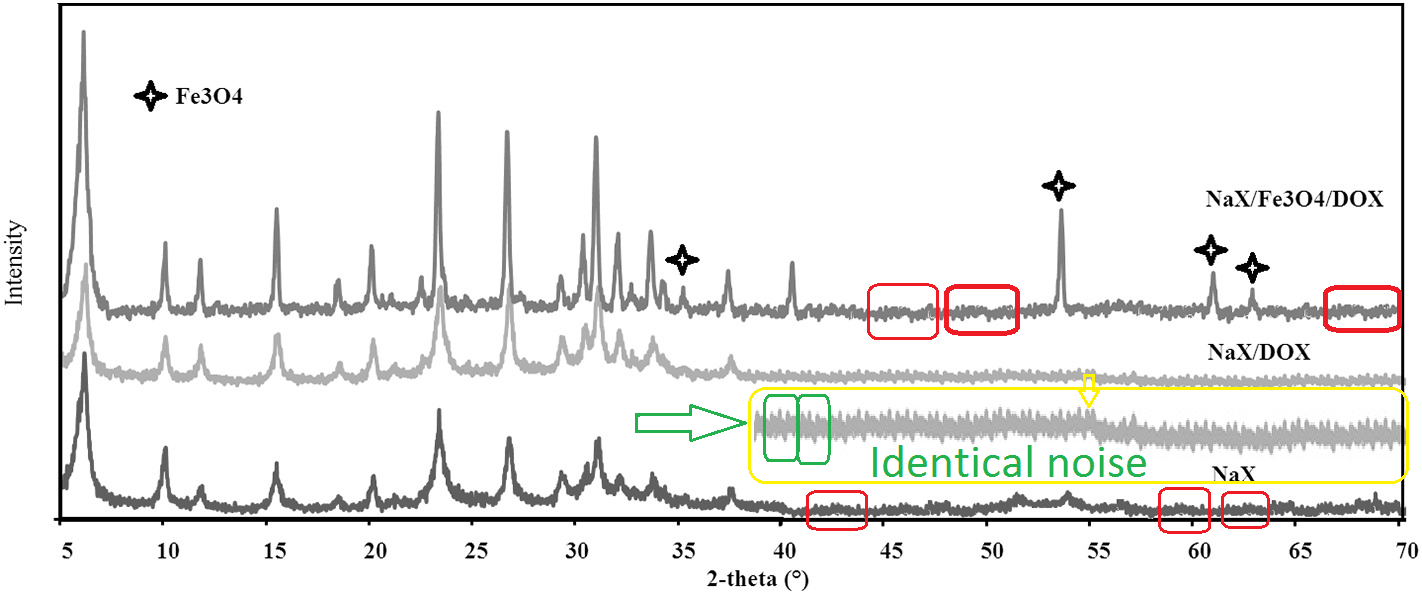
\includegraphics[width=\textwidth]{img/xrd_data_duplication/abasian_figure_1.png}
    \caption*{Regions of unusually similar noise are highlighted by colored boxes. Adapted from a figure created by \href{https://pubpeer.com/publications/DB4037BDC430AFA6C281842E945363\#1}{Tetraphleps parallelus on PubPeer}.}
\end{figure}

\subsection*{Additional resources}

\begin{itemize}
    \setlength\itemsep{-0.5em}
    \item \href{https://osf.io/n8fvw}{COSIG: Extracting vector graphics from a PDF}
    \item \href{https://osf.io/547re}{COSIG: Image duplication}
    \item \href{https://osf.io/g23pf}{COSIG: Software for image forensics}
    \item \href{https://osf.io/hf7qy}{COSIG: X-ray diffraction patterns - Scherrer's equation}
\end{itemize}

\textit{This work made use of the \href{http://xray.facilities.northwestern.edu/}{Northwestern University Jerome B. Cohen X-ray Diffraction Core Facility (RRID:SCR\_017866)} supported by the \href{https://www.nsf.gov/awardsearch/showAward?AWD_ID=2308691}{MRSEC program of the National Science Foundation (DMR-2308691)} at the \href{https://materials.northwestern.edu/}{Materials Research Center of Northwestern University} and the \href{https://shyne.northwestern.edu/}{Soft and Hybrid Nanotechnology Experimental (SHyNE) Resource (NSF ECCS-2025633)}.}

\end{document}